
\chapter{The LHC and CMS}\label{sec:experiment}
%\chapter{Experimental Setup}\label{sec:experiment}

The measurements presented in this thesis are performed
 on data of proton-proton collisions collected %in 2012 and 2015
 by the Compact Muon Solenoid (CMS) detector and
 provided by the
 Large Hadron Collider (LHC) at the 
 European Center for Nuclear Research (CERN).
The LHC was designed to probe physics at the 
 scale of \TeV and is capable of operating at
 multiple energy scales.
As measured in the CM frame
 of protons colliding inside CMS,
 the LHC operated at
 \s8 \TeV in 2012 and \s13 \TeV in 2015.
The measurement of the \ppwbb cross section 
 is performed using 19.8 \fbinv of integrated luminosity
 collected at \s8 \TeV and 
 the measurement of the \ppzgnng cross section
 and the extensions to set limits on DM models 
 uses 2.3 \fbinv of data collected at \s13 \TeV. 

\section{The Large Hadron Collider}
The LHC is a single-ring, double-bore 
 particle accelerator and collider located 
 on the border of France and Switzerland outside Geneva.
It was built using the existing 26.7 km of tunnels from the
 Large Electron Positron collider and hosts
 four primary experiments, located at four
 interaction points where beams of hadrons are made to cross.
Of the four experiments, two (CMS and ATLAS) are built for 
 studying SM processes and searching for new physics in general,
 one (ALICE) is designed to investigate 
 quark-gluon plasma resulting from 
 the high energy collisions of heavy ions such as lead,
 and one (LHCb) was built for the study of
 b-mesons and CP violation.

\subsection{LHC pre-acceleration}
To accelerate protons to their collision energy,
 a multi-stage procedure is used and 
 the major components of the accelerator infrastructure
 are illustrated in Figure \ref{fig:lhc_complex}.
First, protons are separated from
 electrons in neutral hydrogen gas before
 entering the linear accelerator (LINAC2)
 which brings them up to an energy of 50 \MeV
 using a series of oscillating electric potentials.
In this process, rather than having a continuous 
 stream of accelerating protons, the protons
 are grouped into bunches, and the beam
 retains this structure
 of distinct groups of protons separated by gaps
 throughout the acceleration procedure.
After the LINAC2, protons enter the Proton
 Synchrotron Booster (BOOSTER) where
 they are accelerated to 1.4 \GeV and 
 prepared for injection into the Proton Synchrotron (PS).
Inside the PS, bunches are accelerated to
 26 \GeV before being injected into the
 Super Proton Synchrotron (SPS) where they 
 are further accelerated to 450 \GeV.
After the SPS, bunches of protons are sent into
 the LHC.

\begin{figure}[tb]
\caption[The LCH accelerator complex at CERN]{
 Before protons are released into the LHC
  for final acceleration and collision, they pass through
  the LINAC2, BOOSTER, PS, and SPS, 
  undergoing acceleration %and collimation  
  at each stage.
 }
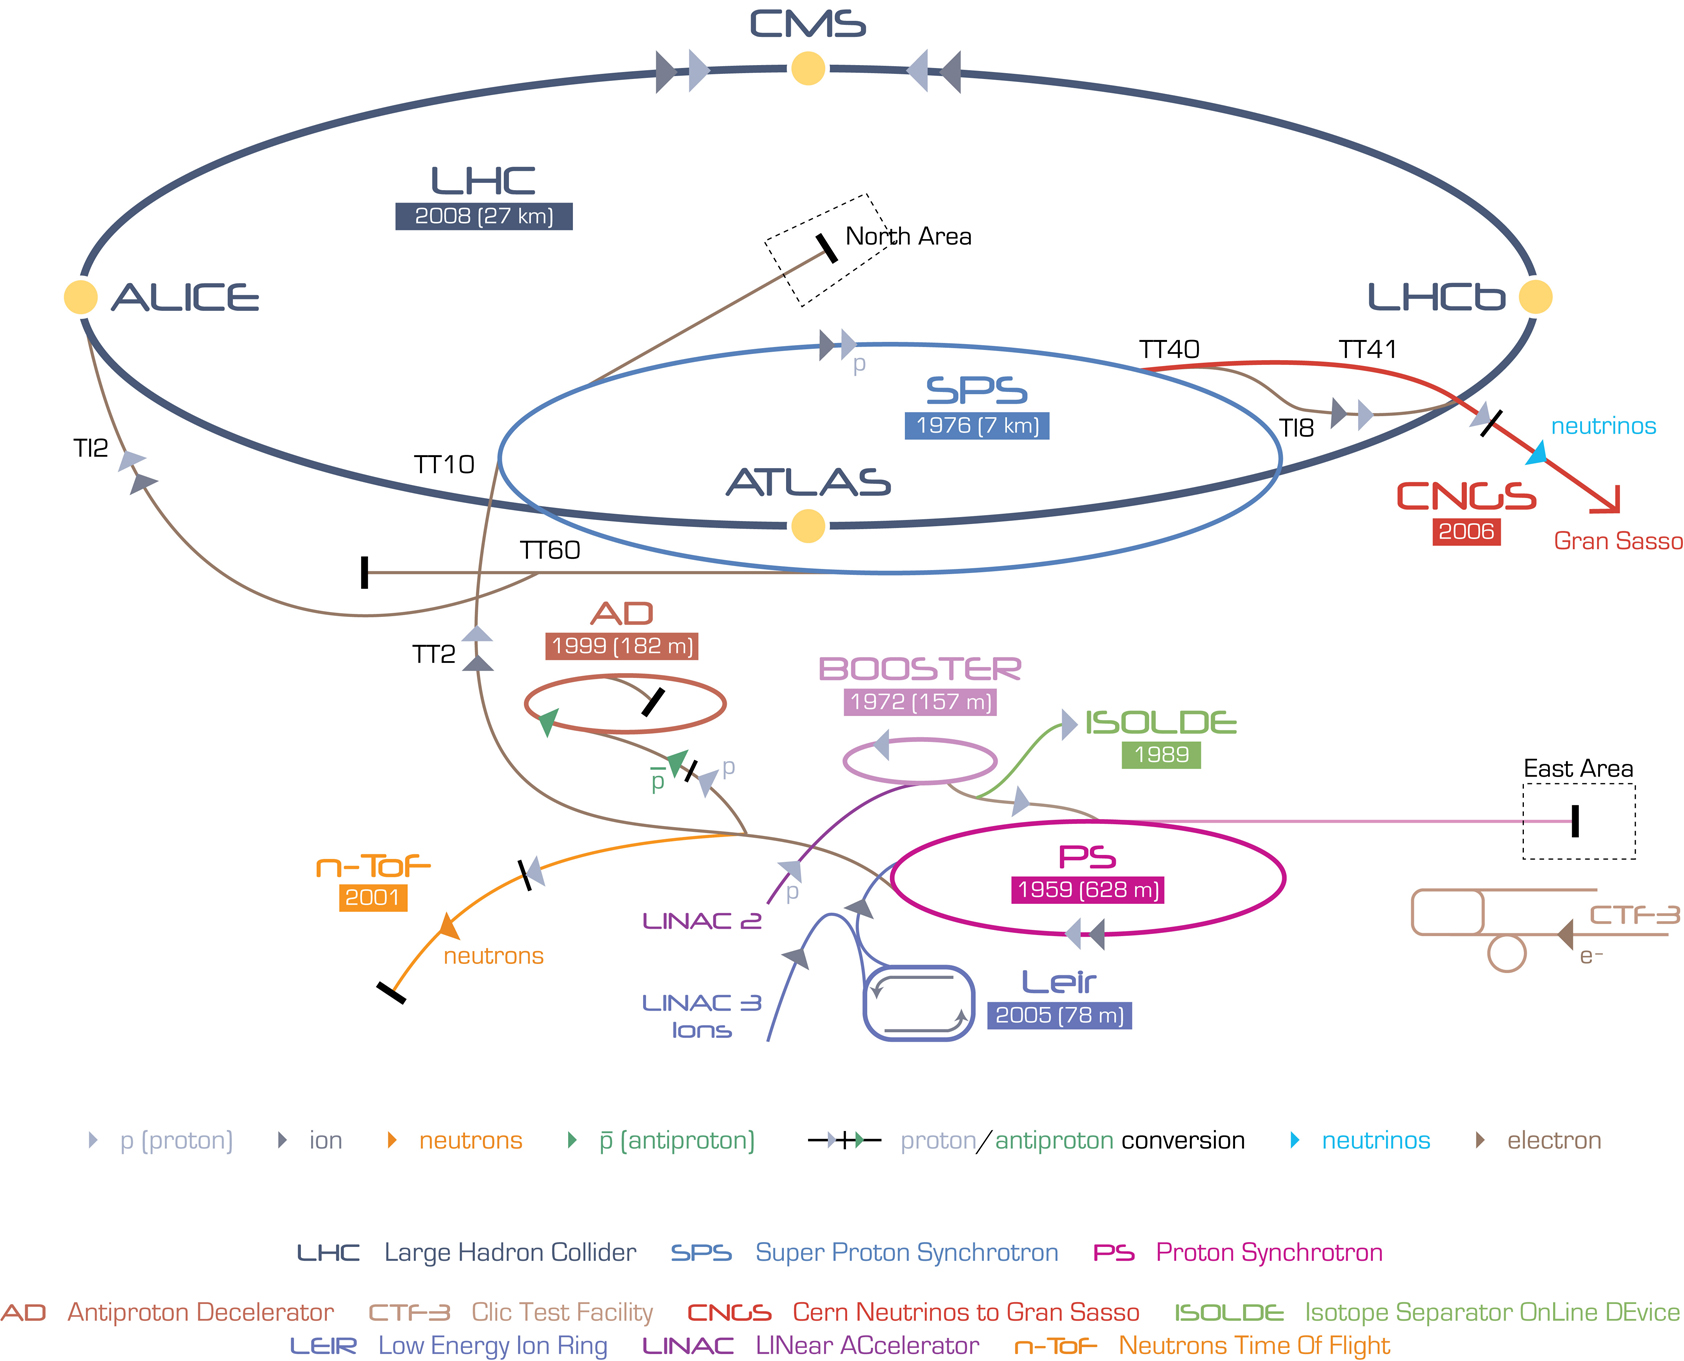
\includegraphics[width=\textwidth]{pdfs/experiment/cern_accelerator_complex.jpg}
\label{fig:lhc_complex}
\end{figure}


\subsection{LHC acceleration}
The work of accelerating and containing
 the protons which %circulate to 
 form %what is known as 
 the beam of
 the LHC is done by superconducting magnets. 
They are cooled to a temperature of 1.9 K
 using liquid helium and are housed in the
 LHC dipole apparatus diagrammed in Figure \ref{fig:lhc_dipole}.
The dipole contains two beam pipes which are
 each surrounded by superconducting coils
 of Niobium Titanium (NbTi)
 which carry oscillating currents when in operation.
These constitute RF cavities
 operating at 400 MHz and having the 
 ability to circulate proton
 bunches in opposing directions 
 between the two beam pipes
 with a spacing of 25 ns between bunches.
The magnets are capable of reaching 
 a strength of over 8 T, a constraint
 imposed by the desired energy scale 
 of the accelerator and the radius of the
 existing LEP tunnels
 in which the LHC was built.  
 
\begin{figure}[tb]
\caption[The LHC dipole]{
 Below is a cross section of the LHC dipole apparatus.
 It contains two beam pipes, each surrounded
  by superconducting magnetic coils
  which are held in place by an iron yolk.
 The system is cooled to a temperature of
  $1.9$ K and is thermally isolated 
  as well as protected from radiation.
 }
%\center
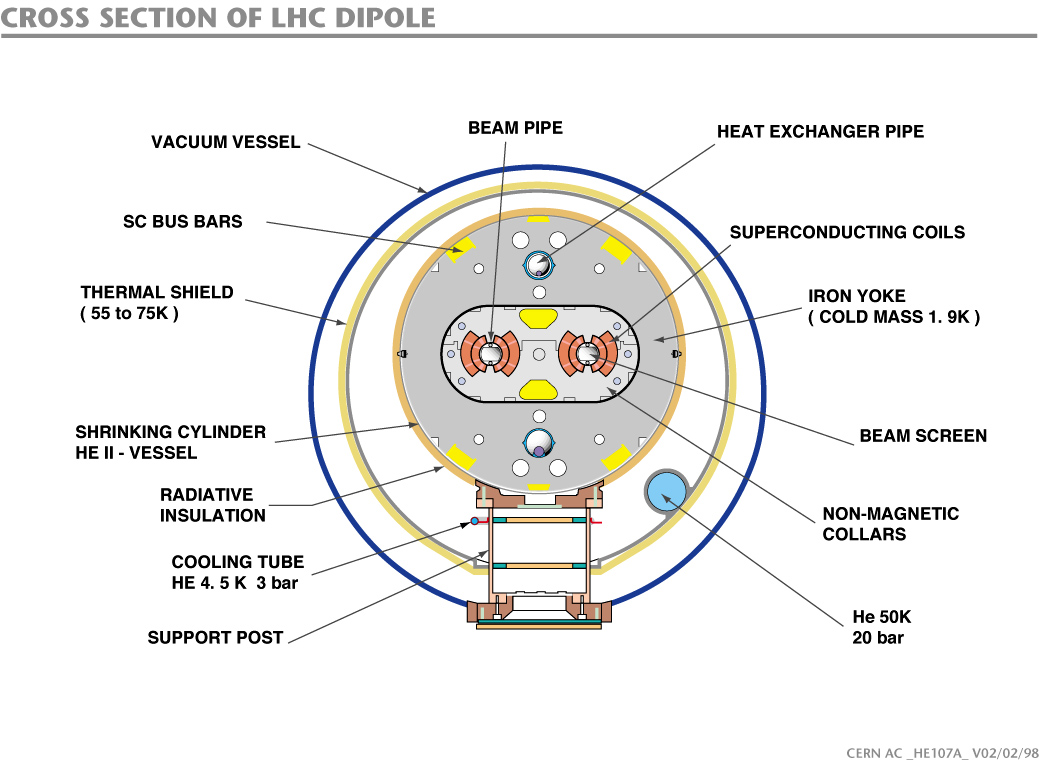
\includegraphics[width=\textwidth]{pdfs/experiment/lhc_dipole.jpg}
\label{fig:lhc_dipole}
\end{figure}

The Lorentz-invariant magnetic force on a
  particle of charge $q$, moving at
  velocity $\mathbf{v}$ in a 
  magnetic field $\mathbf{B}$ is
\begin{equation}\label{eq:bforce}
 \mathbf{B}=q\mathbf{v}\times\mathbf{B}
\end{equation}
 and the relativistic version of Newton's second
 law states
\begin{equation}
 \mathbf{F} = \frac{d\mathbf{p}}{dt} =
  \frac{d}{dt}\left ( \gamma m_0 \mathbf{v}  \right )
\end{equation}
 where $\gamma$ is the relativistic correction
 factor and $m_0$ is the rest mass of the particle.
These can be solved to find that the magnetic field
 required to hold a proton in planar
 circular motion as in the LHC is
\begin{equation}
 \mathbf{B}=\frac{p}{qR}
\end{equation}
 where $R = 4.3$ km.
[todo - unit conversion]

The rate at which a particular collision 
 process occurs
 at the LHC is proportional to 
 the cross section of that interaction
 and the luminosity of the colliding beams
 as given in Equation~\ref{eq:lumidef}.
Assuming a Gaussian beam distribution,
 the machine parameters determine \lumi as

\begin{equation}\label{eq:lumi}
 \lumi=\frac{N_b^2 n_b f_{\mathrm{rev}} \gamma_r}{4\pi\epsilon_n \beta*}\mathcal{F}(\theta)
\end{equation}

 where $N_b$ is the number of particles per bunch,
 $n_b$ is the number of bunches per beam,
 $f_{\mathrm{rev}}$ is the revolution frequency of the bunches,
 $\gamma_r=E_p/m_p$ is the relativistic gamma factor
  for protons at energy $E_p$,
 $\epsilon_n$ is the normalized emittance which 
  characterizes bunch width,
 $\beta*$ is a measure fo the betatron oscillation envelope,
 and $\mathcal{F}(\theta)$ is a relativistic geometrical 
 correction factor which is a function of the
 angle at which the beams cross.
In addition to pushing the energy frontier,
 the LHC also has a significantly greater
 \lumi than previous hadron colliders. 
[Reference to Tevatron]
 
\section{The Compact Muon Solenoid Detector}

The CMS detector was built
 at Interaction Point 5 on the LHC ring
 to collect particle collision data  exploiting the full physics reach
 of the LHC.
The analysis of these data includes
 the discovery of the Higgs boson[REF]
 and high precision measurements of SM processes,
 as well as searches for physics beyond the standard model.
To be able to perform such precision measurements,
 CMS was designed with four main subdetectors 
 that work in concert and with a superconducting solenoid.
The tracking and most of the calorimetric
 detectors are inside the solenoid while
 the muon detectors are outside.
When running, the solenoid produces a 3.8 T 
 uniform magnetic field in its interior,
 and has a uniform 2 T field 
 over the bulk of the detector external to the solenoid.

The innermost of the subdetectors is the tracker
 which uses silicon pixel and strip detectors 
 to record the tracks of charged particles 
 passing through it. 
The tracks are used in conjunction with the
 $3.8$ T magnetic field to measure the momentum of these particles
 and
 this information is used for identifying
 the primary interaction vertex %, defined as
 %the vertex having the highest pt sum of tracks
 as well as locating secondary vertices 
 from the decay of heavy flavor quarks
 such as the b or c.
Outside the tracker is the electromagnetic calorimeter (ECAL), 
 which is designed to have good energy resolution in recording
 the electromagnetic interactions of charged particles
 such as electrons or photons over a wide range of angles.
The hadronic calorimeter (HCAL) is outside the ECAL
 and is designed to absorb energy which
 comes in the form of neutral hadrons and provide 
 good resolution in missing transverse energy, \met.
Outside the calorimeters is the solenoid and steel return yolk,
 and the outermost layers of the detector are dedicated
 to the efficient detection of muons.
The overall length of CMS is 21.6 m, with a radius of 7.3 m
  and a total weight of 12500 tons.

\begin{figure}[tb]
\caption[The CMS Detector]{
 The CMS detector consists primarily of a tracker
  and electromagnetic and hadronic calorimeters
  which are mostly located inside a 3.8 T field provided
  by a superconducting solenoid,
  as well as a muon detection system located 
  outside the solenoid.
 }
%\center
\includegraphics[width=\textwidth]{pdfs/experiment/cms_explode.pdf}
\label{fig:cms_explode}
\end{figure}


 \subsection{Geometry} 
The coordinate system used by CMS is one in
 which the z-axis is aligned with the beam pipe,
 the y-axis is pointing upward vertically
 and the x-axis points radially inward toward the
 center of the LHC ring. 
The detector itself is mostly cylindrically symmetric
 about the beam pipe so cylindrical coordinates
 are also used.
In this system, $r$ is the radial distance
 as measured from the beam pipe, the azimuthal angle, $\phi$,
 is measured up from the x-axis in the x-y plane,
 and the polar angle, $\theta$, is measured
 down from the z-axis.
The angle $\theta$ is commonly replaced by pseudorapidity, 
\begin{equation}\label{eq:eta}
\eta = -\mathrm{ln}(\tan \theta/2)
\end{equation}
 since the distribution of particles
 is roughly constant as a function of $\eta$.
For the calorimeters, “barrel” refers to the region of $|\eta| < 1.4442$,
 and “endcap” to the region $3.0 > |\eta| > 1.566$.
Instrumentation cables are run through the
 gap between the barrel and endcap,
 so this area has detecting components. 
The HCAL forward region covers $3.0 < |\eta| < 5$ and
 the tracker extends to $|\eta| < 2.5$.

 \subsection{Magnet}
To precisely measure the momentum of a charged particle, 
 it is necessary to measure radius of curvature 
 of that particle as it moves through a magnetic field.
The momentum resolution varies as 

\begin{equation}\label{eq:res_mag}
\frac{\delta p}{p} \sim \frac{1}{L^2B}
\end{equation}
 where $L$ is the length of the track of the 
 particle through a magnetic field of
 strength $B$.
For particles at high energy, this requires a very strong
 magnetic field which is achieved by the superconducting 
 solenoid in CMS.
The solenoid operates at 3.8 T with 
 a bore of 3 m in radius and 12.5 m in length
 and is constructed from four layers of NbTi superconductor.
The steel yoke which provides physical support for the 
 CMS structure and serves as an absorber for the
 muon system is fully saturated by the fringe magnetic field
 from the solenoid.

 \subsection{Tracking System}
The inner tracking system of CMS is designed to provide
 precise and efficient measurements of the trajectories
 of charged particles produced during collisions,
 as well as a precise reconstruction of secondary vertices.
The tracker has a length of 5.8 m and a radius of
 1.25 m in a cylindrical structure surrounding the 
 interaction point, as illustrated in Figure \ref{fig:tracker}.

At the core of the tracker and closest to the beam line
 are three concentric cylindrical layers %4.4, 7.3, 10.2 cm 
 of hybrid pixel detector modules which are complemented
 by two discs of pixel modules on each end
 and extend a to a distance of 10 cm from the beam line.
[TODO - Explain - silicon]
In total, the pixel component of the tracker covers
 an area of about 1 m$^2$ with 66 million pixels.
External to the pixel detector are the tracker inner barrel and discs (TIB/TID)
 which are made from silicon strips and extend 
 out to a distance of 55 cm.
There are four layers of strips in the TIB, with 3 discs at each end.
The tracker outer barrel (TOB) is composed of
 6 layers of micro-strip sensors and extends
 in z between $\pm$118 cm and to a radius of 116 cm.
At the end of the z range for the TOB are the
 tracker end caps (TEC) which cover the ranges
 $124<|z|<282$ cm and 22.5 cm $<r<$113.5 cm.
Each TEC is composed of 9 discs,
 each carrying up to 7 rings of silicon micro-strip detectors.
In total, the tracker contains 9.3 million strips
 which cover an area of 198 m$^2$ and extends
 to an acceptance of $|\eta|<2.5$.
For tracks with momentum on the order of 100 \GeV,
 the momentum resolution is around 1-2\% up to $|\eta|<1.6$
 and degrades to around 10\% with increasing $\eta$.

\begin{figure}[tb]
\caption[The CMS Tracking System]{
 Below is a schematic of the CMS tracking system
  where each line represents a detector module.
 The system is made from silicon pixels and
  silicon microstrips distributed into four sections,
  TIB, TID, TOB, TEC.
 }
%\center
\includegraphics[width=\textwidth]{pdfs/experiment/cms_tracker.pdf}
\label{fig:tracker}
\end{figure}
 

 \subsection{Electronic Calorimeter}

The electronic calorimeter (ECAL) is a homogeneous
 calorimeter made from nearly 76000 crystals of lead tungstate (\pbw)
 mounted in the barrel and endcap sections with a 
 preshower detector located in front of the endcaps,
 arranged as shown in Figure \ref{fig:ecal}
In the barrel, avalanche photodiodes are used as photodetectors, 
 and in the endcap vacuum phototriodes are used. 
The material \pbw was chosen for its properties of being
 dense, optically transparent and radiation hard. 
The radiation length inside the ECAL is typically less than 1 cm
 with a Moliere radius of 2.2 cm and about 80\% of the
 light is emitted from a crystal within the first 25 ns.
Since the length of a given crystal is on the order of 20 cm,
 most photons and electrons deposit all of their energy 
 within the ECAL, and do not reach the HCAL.

The use of \pbw crystals allows for excellent position and timing resolution
 with the energy resolution given by 

\begin{equation}\label{eq:ecal_res}
 \left(\frac{\delta_E}{E}\right) =  \left(\frac{2.8\%}{\sqrt{E}}\right)^2 + \left(\frac{0.12}{E}\right) + (0.30\%)^2 .
\end{equation}
 
In this expression, the first term comes from the statistical error 
 in the measurement which arises
 from the stochastic nature of electromagnetic shower evolution
 and the second term represents the error in the measurement
 which results from noise in the electronics or
 energy deposits from additional soft interactions.
The ECAL provides stable and accurate
 measurements of energies over a range from 1 \GeV to 1 \TeV, 
 with the upper limit set by the energy at which electromagnetic showers
 penetrate through the ECAL into the HCAL.
[REF][TODO - how much?]
With time, after undergoing a heavy bombardment of high energy radiation,
 the \pbw crystals physically deteriorate and develop 
 nonuniform light transmission properties.
[REF] 
This is monitored and corrected for using a laser calibration system
 that probes for changes in crystal transparency.
 %during the running of the LHC.

\begin{figure}[tb]
\caption[The CMS Electromagnetic Calorimeter]{
 Below is a diagram of the ECAL, 
  which sits between the tracker and HCAL in CMS.
 It is made from \pbw crystals throughout the volume
  with avalanche photodiodes in the barrel
  and vacuum phototriodes in the endcaps.
 }
%\center
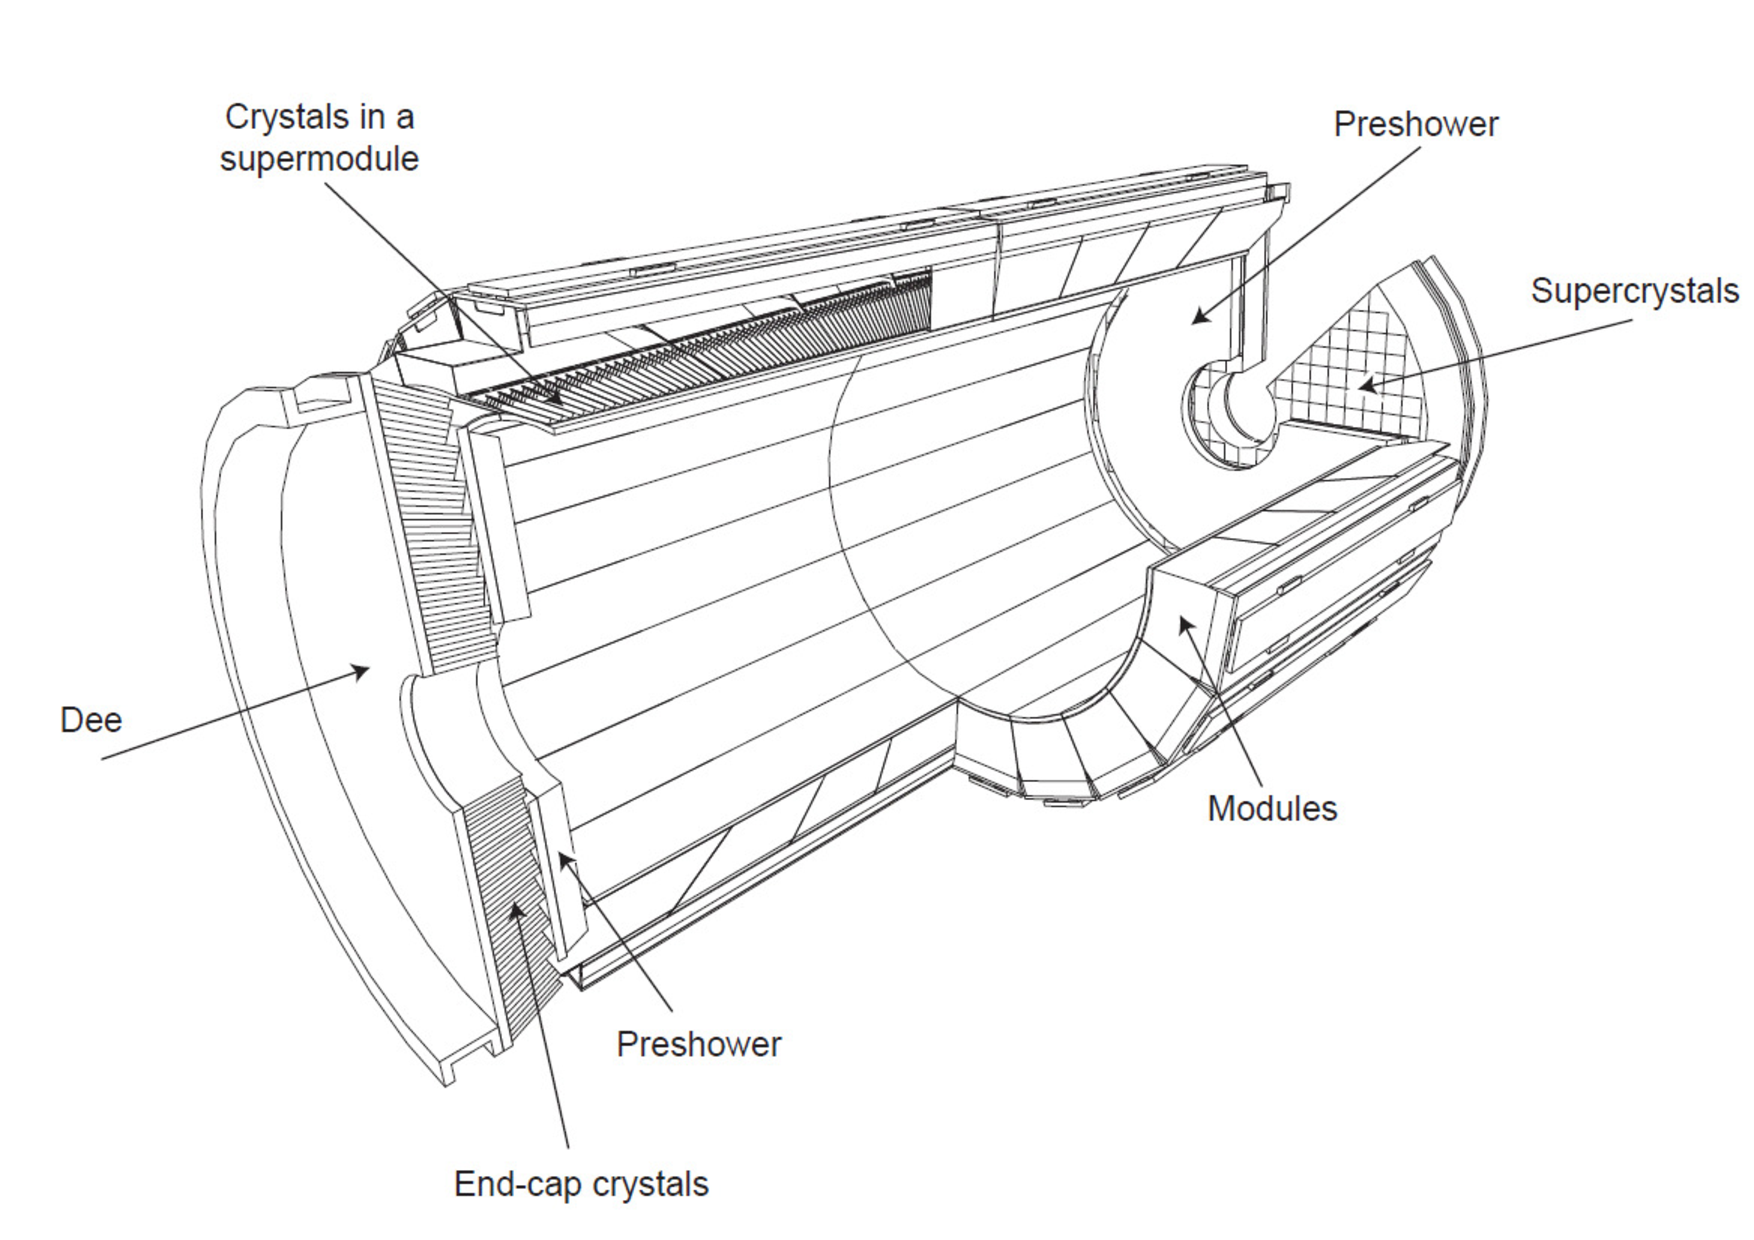
\includegraphics[width=\textwidth]{pdfs/experiment/cms_ecal.pdf}
\label{fig:ecal}
\end{figure}
 

 \subsection{Hadronic Calorimeter}
Situated mostly between the ECAL and the superconducting solenoid
 is the hadronic calorimeter (HCAL) which plays a
 crucial role in the measurement of hadron jets
 and particles such as neutrinos which escape the detector
 and result in apparent missing transverse energy.
The HCAL is designed to contain the energy of neutral
 particles which pass through the ECAL and is therefore made
 from dense materials such as 
 steel and brass interleaved with scintillating material.
Because the HCAL is designed to fit between these
 two components, it takes the shape of a hollow
 cylinder of inner radius 1.77 m and outer radius 2.95 m
 and one half of the HCAL is illustrated in Figure \ref{fig:hcal}.

The barrel of the HCAL (HB) extends to $|\eta|<1.3$ 
 and is constructed from brass absorber plate wedges aligned parallel 
 to the beam axis and mounted in an overlapping configuration,
 with a smaller amount of steel used in the inner and outermost
 wedges for structural stability.
The endcap of the HCAL (HE) extends this coverage to $|\eta|<3.0$
 and is complemented by the forward hadron calorimeter (HF)
 which is made from the comparatively radiation-hard 
 steel plates embedded with quartz fibers.
Inside the barrel region there is an additional layer of the
 HCAL, the outer calorimeter (HO), which is located just
 outside the solenoid and uses it as an absorber 
 for energetic showers which start late in the HB.

In the HB, HO and HE, light from particle showers
 [TODO - not exactly ..] 
 inside scintillators and collected by quartz fibers
 and then used as an estimate of the total energy of the shower.
In the HF, this estimate is made using the Cherenkov 
 radiation from particles with energy above 190 \keV
 collected by the quartz fibers.
For the two cases, the energy resolution takes the same
 functional form 

\begin{equation}\label{eq:hcal_res}
 \left(\frac{\delta_E}{E}\right) =  \left(\frac{A}{\sqrt{E}}\right)^2 + (B)^2 
\end{equation}
 where $A$ is 90$\%$ (172$\%$) in the HB/HO/HE (HF)
  and relates to the stochastic uncertainty of shower evolution
 and $B$ is 4.5$\%$ (9.0$\%$) and comes from uncertainties in calibration.


\begin{figure}[tb]
\caption[The CMS Hadronic Calorimeter]{
 A schematic layout of the HCAL, which complements the ECAL
  in providing a measurement of the total energy produced 
  in a collision.
 The HCAL is made from brass and steel plates,
  embedded with quartz fibers.
 }
%\center
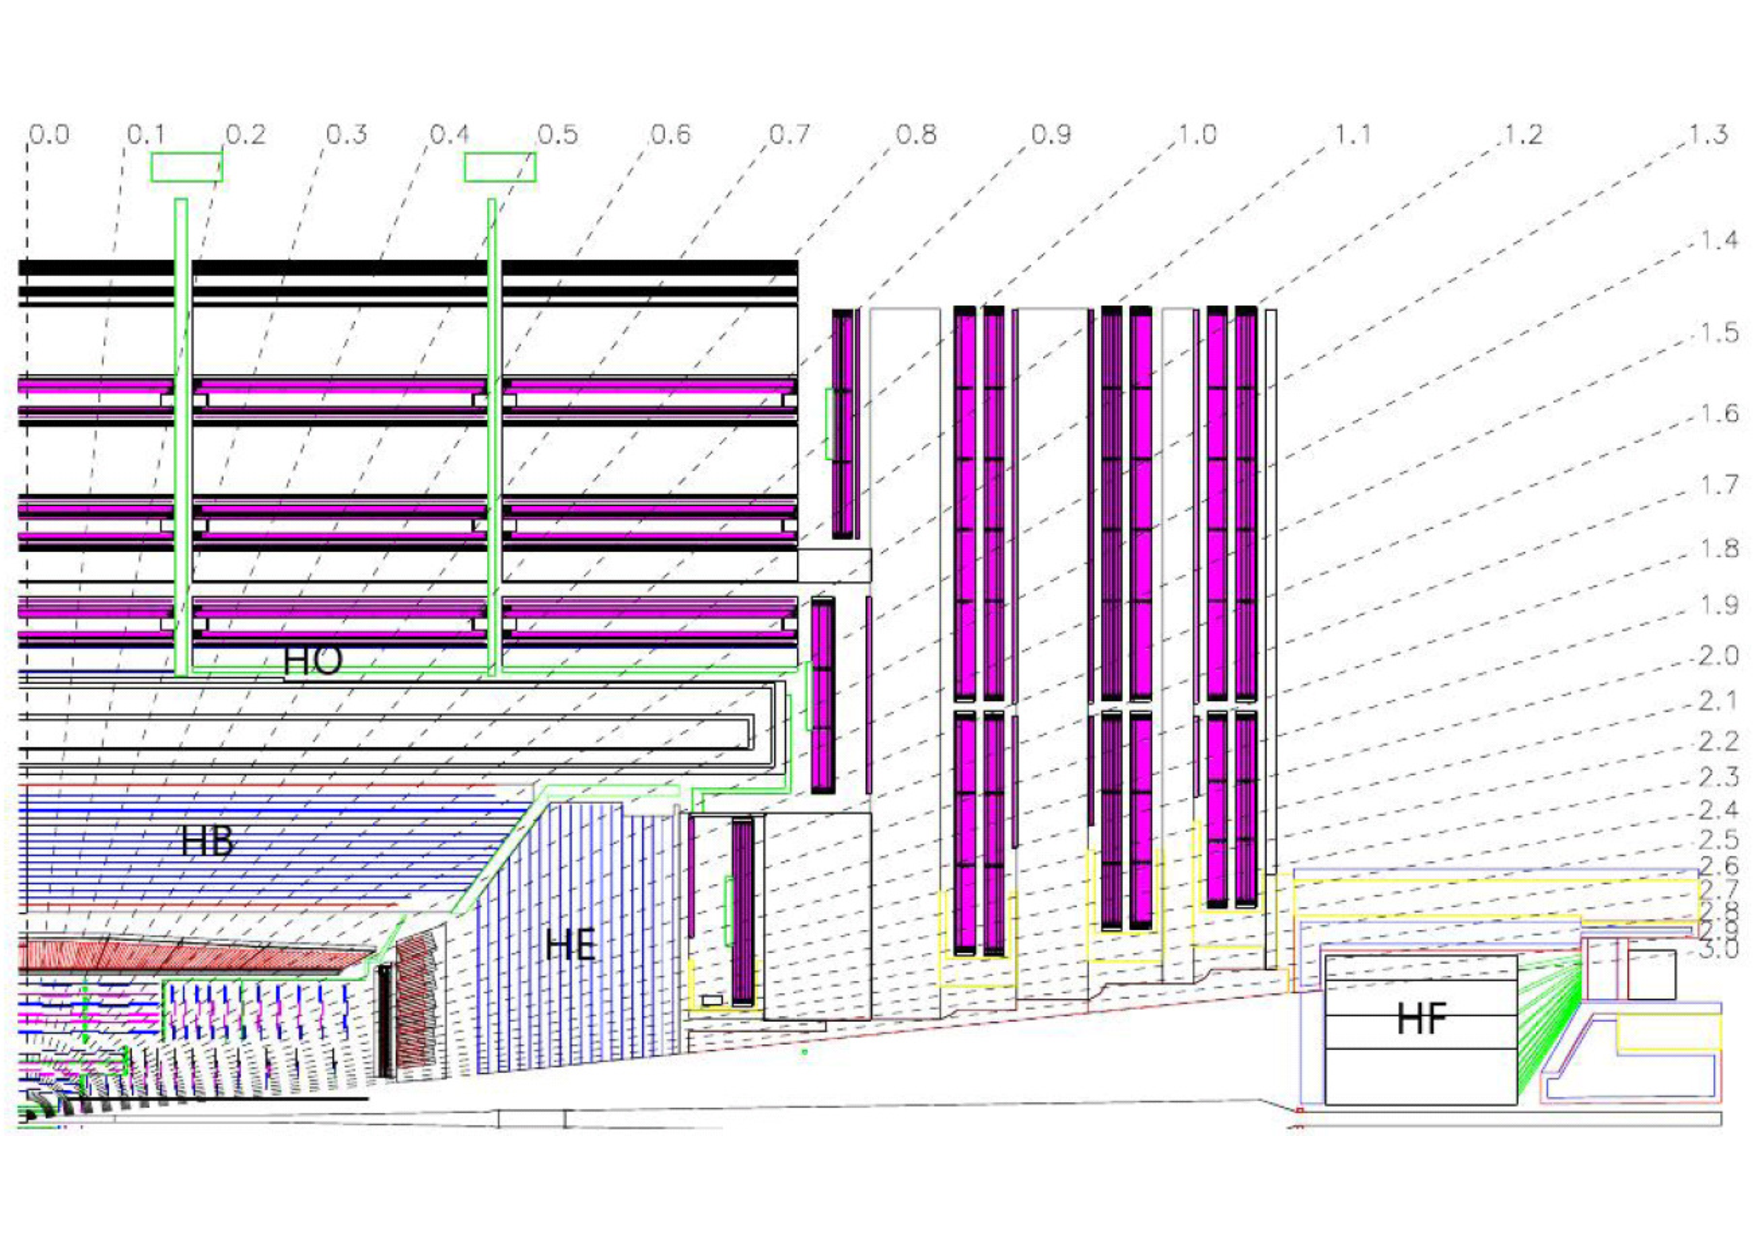
\includegraphics[width=\textwidth]{pdfs/experiment/cms_hcal.pdf}
\label{fig:hcal}
\end{figure}
 

 \subsection{Muon System}

Muons play a central role in the physics program outlined
 by CMS and the muon detection system is positioned 
 as the outermost layer of the detector. 
Unlike the other charged leptons, 
 muons typically pass through the ECAL and HCAL and
 deposit only a fraction of their energy, so
 a dedicated muon system is necessary in order to
 determine the momentum of these particles.
The muon system is composed of three different kinds
 of gaseous detectors,
 drift tubes (DTs), resistive plate chambers (RPCs)
 and cathode strip chambers (CSCs) and their layout is
 illustrated in Figure \ref{fig:muon}.

The barrel region of the muon system is covered by DTs
 in the range $|\eta|<1.2$ and the endcaps are covered 
 by CSCs in the range $0.9<|\eta|<2.4$.
The RPCs are located
 in the range $|\eta|<1.6$ and provide fast,
 independent and highly segmented transverse
 momentum measurements of muons. 

The DT system is composed of 4 stations which 
 form concentric cylinders about the beam line
 and contain 172000 sensitive wires. 
As charged particles enter the DTs,
 they ionize the Ar/CO$_2$ gas mixture,
 knocking off electrons  which 
 then are attracted to the positively charged wires.

The CSCs are less sensitive to uneven magnetic fields
 and high particle rates so are therefore used in the endcaps.
They are made from crossed arrays of positively 
 charged wires and negatively charged strips
 in gas and are composed
 of six layers, giving them precise timing
 as well as positional information. 
As an upgrade between the 2012 and 2015 data taking periods,
 a fourth layer of CSCs was added to the CMS detector, 
 adding to the three which were present in 2012.

The RPCs are built from two sheets held at opposite
 charges and separated by a gas volume.
As muons move through the chamber, electrons
 are ionized from the gas and attracted to small
 metallic strips which they reach after a small
 but well known time delay. 
The timing resolution of RPCs is on the order of 1 ns. 

\begin{figure}[tb]
\caption[The CMS Muon System]{
 The CMS muon system uses DTs, RPCs,
  and CSCs to provide muon detection
  up to $\eta < 2.4$.
 Shown below is the geometrical arrangement
  of the different muon
  subsystems and how they fit with
  the rest of the CMS detector.
 }
\label{fig:muon}
%\center
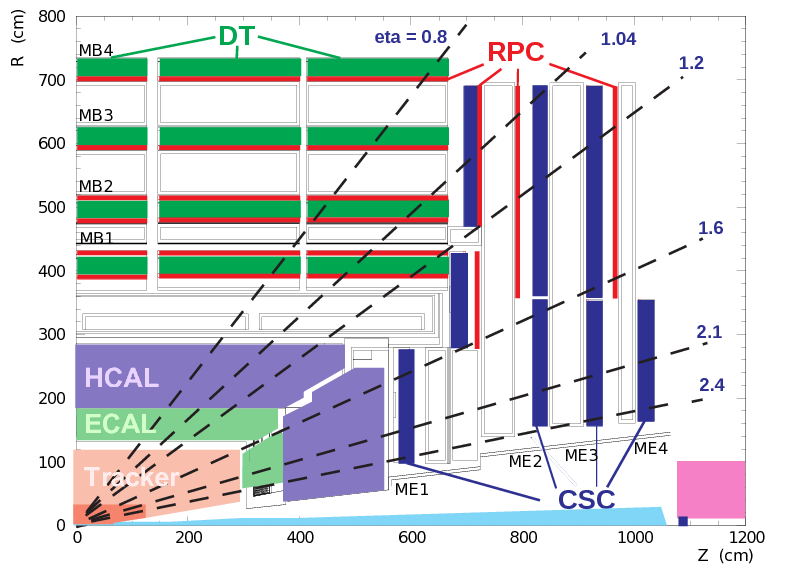
\includegraphics[width=\textwidth]{pdfs/experiment/cms_muon.png}
\end{figure}
 
 %\subsection{Trigger System}


